\section{Probing radiation}

This work is focussed on the use of X-ray and neutron scattering, therefore it is pertinent to discuss how each of these probing radiation is produced and detail the advantages of each with resepect to the other.

\subsection{Generation of X-rays}

X-rays are a form of electromagnetic radiation similar to visible light, albeit with a much shorter wavelength, from \SI{0.01}{\nano\meter} to \SI{10}{\nano\meter}. There are three common ways to produce X-rays; two are available within the laboratory, while the other is exclusive to large scale facilities.

The two laboratory source X-ray generation techniques are the X-ray tube and the rotating anode. An X-ray tube consists of a filament and an anode within a vacuum chamber, by passing a high voltage electrical current across the filament electrons are emitted which accelerate towards the anode. On collision with the anode, the rapid deceleration results in the emission of X-rays of a characteristic wavelength based on the anode material.\cite{Schnablegger2017} The most common material for an X-ray tube anode is copper which gives off radiation of about \SI{8}{\kilo\eV}.

The other common laboratory method for the generation of X-rays is the rotating anode, which is an improvment on the X-ray tube. In the X-ray tube, each time that an electron contacts the anode there is some energy transfer, this means that over many millions of collisions, the temperature of the anode can raise significantly, leading to a temperature limitation on the X-ray flux available. This lead to the development of the rotating anode, this is simply where the anode is made from a rotating wheel, so that the bombardment is spread across the whole wheel reducing the energy localisation. This allows an increase in the photon flux by about an order of magnitude.\cite{Schnablegger2017}

The third method of X-ray generation is at a synchrotron facility, this method has the drawback that it requires access to a national or international faciliy; such as Diamond Light Source (DLS) or the European Synchrotron Radiation Facility (ESRF). The way in which X-rays are generated at the synchrotron involves the acceleration of an electron, rather than the deceleration as with the laboratory sources. This is achieved by having relativistic electrons travel in around a curve, from Newtonian mechanics it is known that travelling on a curve at constant speed is equivalent to acceleration. This is achieved by firstly accelerating the electrons, produced in an linear accelerator (Linac), to near the speed of light in a booster synchrotron before injecting them into the storage ring. In the storage ring, the electrons are kept at relativistic speeds with bending magnets (BM) and straight sections making up a ring (Fig.~\ref{fig:syn}). The circularity of the ring is dependent on the number of bending magnets that make up the ring; for example, DLS has 48 bending magnets with 48 straight sections.
%
\begin{figure}
	\centering
	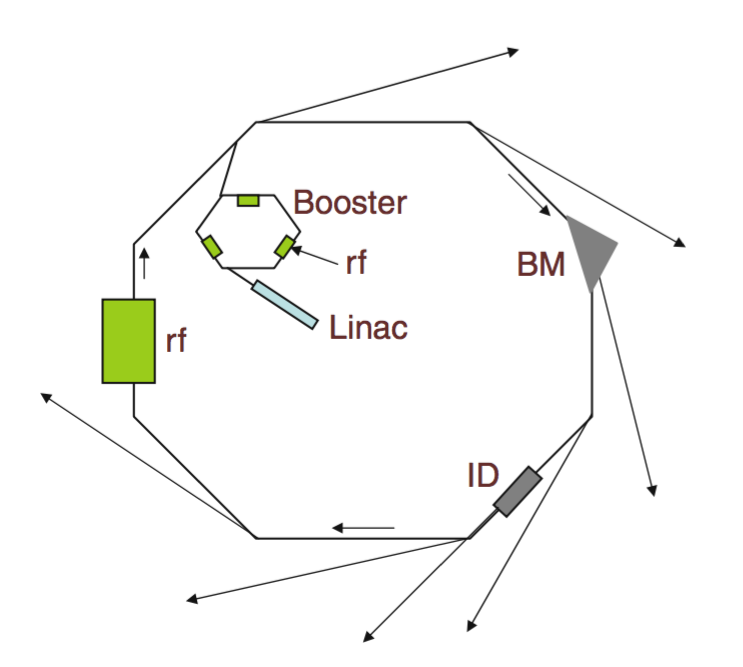
\includegraphics[width=0.85\textwidth]{theory/syn}
	\caption{A schematic representation of a synchrotron radiation source, identifying the Linac, the booster ring, the radio-frequency cavities (rf), the bending magnet (BM) and the insertion device (ID), from Ref.~\cite{Garcia-Gutierrez2009}. Reprinted/adapted by permission from Springer Nature Customer Service Centre GmbH: Springer Nature Bases of Synchrotron Radiation, Light Sources, and Features of X- Ray Scattering Beamlines by M.C. Garc\'{i}a-Guti\'{e}rrez, D.R. Rueda\textsuperscript{\textcopyright} (2009).}
	\label{fig:syn}
\end{figure}
%

When an electron accelerates (or travels on a curve), Cherenkov radiation is emitted in accordance with the Cherenkov relation,
%
\begin{equation}
	n_i\beta_c\cos{\theta_e} = 1,
\end{equation}
%
where, $n_i$ is the refractive index for the dielectric medium, $\beta_c$ is the fraction of the speed of light at which that electron is travelling, and $\theta_e$ is the angle between the electron trajectory and the trajectory of the resulting photon \cite{Garcia-Gutierrez2009}. The curve is the result of a bending magnet, meaning that at each bending magnet there can be a beamline which gives out synchrotron light. The light this is given off from a bending magnet is continuous and broad, covering a wide range of the electromagnetic spectrum. The alternative to a bending magnet beamline is a beamline which is served by an insertion device (ID). An insertion device is able to offer more specific radiation characteristics (photon energy, narrower band) than a bending magnet, and are placed on the magnet-free straight sections of the synchrotron. Common insertion devices include wavelength shifters, wigglers, and undulators.

The type of insertion device that is present at both I07 and I22 at DLS is an undulator. An undulator consists of a series of magnets of opposing polarity whihc causes the electrons to `wiggle' back and forth (Fig.~\ref{fig:undulator}). This results in a superposition of radition from $N_P$ sources, where $N_P$ si the number of magnets, yielding quasi-monochromatic radiation. The brilliance of different X-ray sources are compared in Table \ref{tab:sources}, this shows the significant benefit that an undulator offers in terms of photon brilliance.
%
\begin{figure}
	\centering
	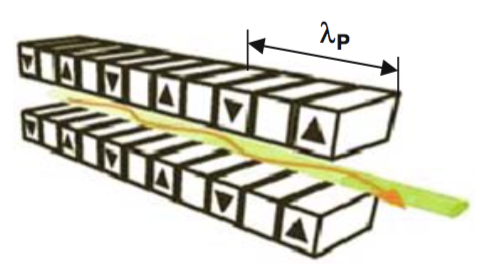
\includegraphics[width=0.85\textwidth]{theory/undulator}
	\caption{A diagram of an undulator insertion device such as that on I07 or I22 where $\lambda_P$ is the period length between opposing magnets, from Ref.~\cite{Garcia-Gutierrez2009}. Reprinted/adapted by permission from Springer Nature Customer Service Centre GmbH: Springer Nature Bases of Synchrotron Radiation, Light Sources, and Features of X- Ray Scattering Beamlines by M.C. Garc\'{i}a-Guti\'{e}rrez, D.R. Rueda\textsuperscript{\textcopyright} (2009).}
	\label{fig:undulator}
\end{figure}
%
%
\begin{table}
	\centering
	\caption{A comparision of the photon brilliance from different light sources, adapted from Ref.~\cite{Sivia2011}.}
	\label{tab:sources}
	\begin{tabular}{l | c}
		\toprule
		\multirow{2}{*}{Light source } & Approximate brilliance/ \\
 & \si{photons\,\second^{-1}\milli\radian^{-2}{0.1}\percent bandwidth^{-1}} \\
		\midrule
		Candle & $10^5$ \\
		X-ray tube & $10^8$ \\
		Sun & $10^{10}$ \\
		Bending magnet & $10^{15}$ \\
		Undulator & $10^{20}$ \\
		\bottomrule
	\end{tabular}
\end{table}

\subsection{Generation of neutrons}

Neutrons hold an advantage over X-rays, particularly for application to the study of soft matter, in the ability to utilise contrast variation to increase the quantity of information from the sample, this is discussed in deatil in Section \ref{convar}. However, neutrons cannot be produced safely on a laboratory scale, therefore it is always necessary to visit large scale facilities to harness neutrons for scattering experiments. These facilities come in two flavours; the reactor source and the spallation source, each offering unique benefits.

Neutron reactor sources, such as the Institut Laue-Langevin (ILL) in Grenoble, France, as currently the most common format of neutron source and are capable of producing the highest average neutron flux, the number of neutrons per second per unit area, for example the High-Flux Reactor at the ILL is capable of producing a neutron flux of \SI{1.5E15}{neutrons\,\second^{-1}\centi\meter^{-2}}.\cite{ill2016} A reactor source operates on the principle of nuclear fission, where an atomic nucleus is capable of breaking down into smaller nuclei, overcoming the strong nuclear force. This often involves using uranium enriched with its fissile isotope, \ce{^{235}U}, which after the initial absorption of a stray neutron, from a cosmic ray, or spontaneous fission, will undergo fission to release, on average, 2.5 daughter neutrons, an example of a possible uranium fission mechanism is:
%
\begin{equation*}
	\ce{n + ^{235}U -> ^{236}U -> ^{134}Xe + ^{100}Sr + 2n}.
\end{equation*}
%
This type of mechanism is the basis for research, and nuclear power, reactors.\cite{Sivia2011} One of the major drawbacks for reactor neutron sources is the percieved public opinion towards such facilities. Major saftey concerns, such as ``nuclear meltdown'' and the resulting nuclear waste, mean that reactor souces are often unpopular and therefore struggle to obtain funding required for operation.

The other form of neutron source is a spallation source, this is much less controversial as it does not require fissile materials and hence there is no risk of a nuclear disaster. The ISIS neutron and muon source (Oxfordshire, UK) is an example of a spallation source, where high energy protons, \SI{800}{\mega\eV},\cite{isis2016} are accelerated towards a tungsten target. When the protons strike the target, they can cause the release of a series of neutrons, the first batch of neutrons are given off with too high an energy to be useful, however, less excited neutrons are given off by secondary emissions. In addition to the public preception benefit, spallation sources also have a technological advantage in the time-of-flight technique. The time-of-flight (ToF) technique is based on the fact that at a spallation source, it is possible to know the time at which the neutron was ejected by the target to a high level of precision and accuracy, and therefore it is possible to measure the time taken for the neutron to reach the instrument. Since the neutron is a particle of a finite mass, $m$, it is possible to correlate the velocity, $v$, of the particle with the kinetic energy, $E_k$,
%
\begin{equation}
	E_k = \frac{mv^2}{2},
\end{equation}
%
and with knowledge of the energy of the particle, its wavelength $\lambda$, can be determined by the de Broglie relation,
%
\begin{equation}
	E = h\omega = \frac{hv}{\lambda},
\end{equation}
%
where, $h$ is Planck's constant and $\omega$ is the neutron frequency. Therefore, the wavelength of the neutron is proportional to the inverse of the particle's velocity, and hece the time-of-flight, $t_F$,
%
\begin{equation}
	\lambda = \frac{h}{mv} = \frac{ht_F}{mL_F},
\end{equation}
%
where, $L_F$ is the distance between the target and the instrument. The fact that the neutrons can spread out in the flight from the target means that wavelength-dispersive techniques, where the neutron wavelength is measured rather than the scattering angle, are possible at spallation sources which cannot be carried out at reactor sources. The negative side-effect of current spallation sources is that they have a lower average flux than reactor sources, however the building of the European Spallation Source (ESS) will change this as it offers an average flux similar to that of a reactor source, but with the benefits of the spallation technique.

A problem that is inherent for both reactor and spallation sources is that the energy of the neutrons given off is usually too high to be used to study condensed materials, such as soft matter. This means that moderation must be used to reduce the energy of the neutrons passing through the sample. The neutrons which are considered to be optimal for the study of condensed materials are thermal neutrons, named because their energy is appromately that of ambient temperature. Thermal neutrons are achieved by allowing the neutrons to pass through a large volume of moderator material, usually graphite or heavy water (\ce{D2O}), stored at \SI{300}{\kelvin} before they reach the instrument.\cite{Sivia2011}

\subsection{Contrast variation}
\label{convar}

The scattering profile generated by the interaction of some system with radiation depends on three factors:
%
\begin{itemize}
	\item the spatial arrangement of the atoms in the system,
	\item the instrument being used to measure the pattern; instrumental resolution function, and
	\item the interaction between the radiation and the matter under investigation.
\end{itemize}
%
This final factor is perhaps better known as the `scattering contrast', this is an extremely important factor in the study of soft matter, particularly when the probing radiation is the neutron. The scattering contrast makes it possible to select individual components of the system and investigate their structural properties.\cite{Schurtenberger2002} The differential cross-section, $\sfrac{\text{d}\sigma}{\text{d}\Omega}$ of a point scatterer, as shown in Eqn.~\ref{equ:sca}, varies only with respect to the scattering length of the species, $b$,
%
\begin{equation}
	\frac{\text{d}\sigma}{\text{d}\Omega} \propto b^2.
\end{equation}
%
However, as discussed in Section \ref{sec:sld}, it is often easier to use the scattering length density, $\rho$.

When an X-ray interacts with an atom, it is scattered by the interaction with the electrons, this is due to the X-ray being a form of electromagnetic radiation. Furthermore, it means that the scattering length of an atom by an X-ray is directly proportional to the number of electrons in the atom, so it is therefore difficult to discern between the scattering from a carbon atom (6 electrons) and a nitrogen atom (7 electrons), furthermore the scattering from hydrogen atoms is practically non-existent.

The scattering length a neutron by an atom varies unsystematically with respect to the atomic number of a species, this is shown in Fig.~\ref{fig:scatlen}. Furthermore to the apparently random variation with changes in atomic number, there is also significant variation with mass number, e.g. between isotopes of the same atom. This is also dependance due to the magnetic state of the atom, however this is normally unimportant for soft matter. The scattering lengths differ with the nuclear spin energy level, this leads to an average scattering length, $\langle b \rangle$, for isotopes where the nuclear spin is non-zero ($S\neq 0$). There are two forms of scattering, coherent and incoherent, for which the scattering cross-sections, $\sigma$, are determined by,
%
\begin{equation}
	\begin{aligned}
		\sigma_{\text{coh}} & = 4\pi\langle b \rangle ^2 \\
		\sigma_{\text{incoh}} & = 4\pi(\langle b ^ 2 \rangle - \langle b \rangle ^2) \\
	\end{aligned}
\end{equation}
%
The coherent scattering is the scattering from nuclei that all have the same value of $\langle b \rangle$, and leads to the important scattering pattern. Whereas, the incoherent scattering is caused by the `disorder' between the isotopes, and is the cause of the background present in the measurement. Examples of these scattering cross-sections for nuclei relevant to soft matter are shown in Table \ref{tab:crosssec}. It can be seen that the incoherent scattering from the \ce{^1H} nuclei is more than forty times the coherent scattering. This leads to a large, intrusive background present in the scattering pattern of hydrogenous samples.
%
\begin{figure}
	\centering
	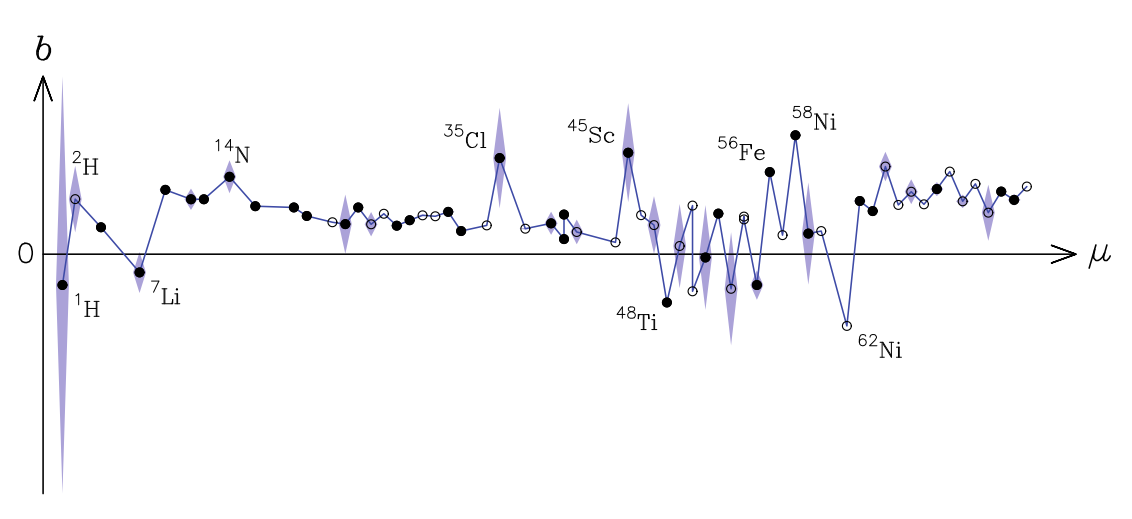
\includegraphics[width=0.85\textwidth]{theory/scatlen}
	\caption{The variation of the average neutron scatteirng length, $\langle b \rangle$ (circles), with atomic mass, $\mu$. The standard deviation, $\Delta b$, is indicated with the shaded regions. Reproduced, with permission of Oxford University Press\textsuperscript{\textcopyright}, from Ref.~\cite{Sivia2011}.}
	\label{fig:scatlen}
\end{figure}
%
\begin{table}
	\centering
	\caption{Examples of coherent and incoherent scattering cross-sections, from Ref.~\cite{Schurtenberger2002}.}
	\label{tab:crosssec}
	\begin{tabular}{r | c c c}
		\toprule
		Isotope & $S$ & $\sigma_{\text{coh}}$/\SI{e-28}{\meter\square} & $\sigma_{\text{incoh}}$/\SI{e-28}{\meter\square} \\
		\midrule
		\ce{^1H} & $\sfrac{1}{2}$ & 1.8 & 79.7 \\
		\ce{^2H} & 1 & 5.6 & 2.0 \\
		\ce{^{12}C} & 0 & 5.6 & -- \\
		\ce{^{14}N} & 1 & 11.6 & 0.3 \\
		\ce{^{16}O} & 0 & 4.2 & -- \\
		\bottomrule
	\end{tabular}
\end{table}
%
The difference between the scattering of \ce{^1H} and \ce{^2H}, evident in Table \ref{tab:crosssec}, can lead to a very useful technique if soft matter scattering, known as contrast variation. The idea of contrast variation is based on the substitution of one isotope of an atom for another, while not introducing significant change to the properties of the material. Traditionally the benefit of this came in terms of contrast matching out a part of the system to reduce the dimensionality of the problem for analysis. For example, by matching the solvent scattering length density to that of the tails of the surfactants at the centre of a micelle there would only be scattering from the heads, and conversely there would only be scattering from the tails if the solvent had the same scattering length density as the head groups. This means that the problem becomes more straightforward as there are fewer variable parameters when fitting the data. This idea is represented graphically in Fig.~\ref{fig:convar}.
%
\begin{figure}
	\centering
	
\includegraphics[width=0.85\textwidth]{theory/convar}
	\caption{The effect of varying the scattering length density of the solvent in a micelle system, (a) the system in pure solvent, (b) the solvent is contrast matched to the surfactant tails, and (c) the solvent is contrast matched to the surfactant heads.}
	\label{fig:convar}
\end{figure}
%
The technique of contrast variation may also be used in terms of data analysis. By increasing the number of data sets corresponding to a single model at different constrasts, the solution for the true sturcture of the model from the scattering data becomes more robust. This is due to the fact that each different contrast can be considered as an independent measurement of the same system, and hence each set of scattering data can be used within the data analysis procedure to obtain the best global agreement to the experiment. This co-refinement of multiple experiments can, under the right conditions, be used to simulatenously consider both neutron and X-ray datasets.\cite{Nelson2006}

There is also the possibility of using contrast variation when the probing radiation is the X-ray, through the use of anomalous scattering. This is where different wavelengths of radiation give different scattering, when the wavelengths are on opposite sides on an X-ray absorption edge. This is not frequenctly used for soft matter species, as the X-ray absorption edges for elements common in soft matter (H, C, N, O, etc.) are at very low X-ray energies so generally outside of the accessible range. \cite{Schurtenberger2002}
